\subsection{Method: Graph Neural Networks (GNNs) for Particle Jets \quad / \quad \textthai{วิธีการ: GNN สำหรับเจ็ตอนุภาค}}
\begin{paracol}{2}
In particle physics, a "Jet" is a spray of high-energy particles produced by quarks or gluons. Traditionally, these were analyzed using high-level variables (e.g., energy, momentum). However, GNNs allow us to treat the entire jet as a **Graph**\index{Graph@กราฟ (Graph)}, where each particle is a node.

\textbf{Message Passing Neural Networks (MPNNs)}\index{MPNNs@MPNNs (MPNNs)} are particularly effective here. By allowing particles to "talk" to their neighbors in energy space, the AI learns the complex relational structure of the particle shower. This is critical for identifying rare signatures like the **Higgs Boson decay**.

As seen in Figure \ref{fig:ch10_tracks}, GNNs can reconstruct the curved paths of particles in a detector with significantly higher fidelity than standard algorithms, even in high-density "Pile-up" environments.

\begin{figure}[ht]
    \centering
    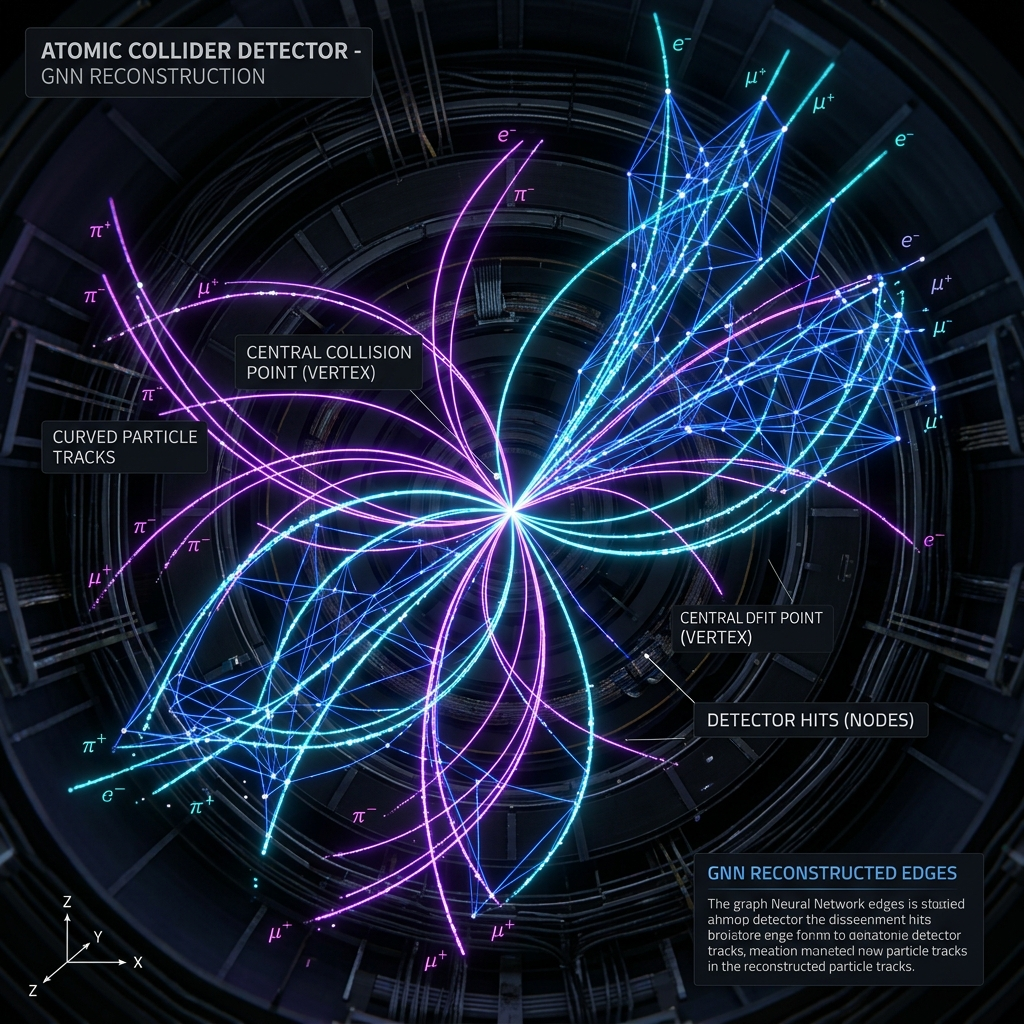
\includegraphics[width=0.9\textwidth]{assets/ch10_results.png}
    \caption{3D Reconstruction of Particle Jets using GNN. The AI identifies the parent quark by analyzing the intricate graph of secondary particle hits.}
    \label{fig:ch10_tracks}
\end{figure}

\switchcolumn

\begin{thai}
ในฟิสิกส์อนุภาค "เจ็ต (Jet)" คือละอองของอนุภาคพลังงานสูงที่เกิดจากควาร์กหรือกลูออน ตามดั้งเดิมแล้ว สิ่งเหล่านี้จะถูกวิเคราะห์โดยใช้ตัวแปรระดับสูง (เช่น พลังงาน โมเมนตัม) อย่างไรก็ตาม GNN ช่วยให้เราสามารถมองเจ็ตทั้งหมดเป็น **กราฟ (Graph)** โดยที่อนุภาคแต่ละตัวคือโหนด

**Message Passing Neural Networks (MPNNs)** มีประสิทธิภาพเป็นพิเศษในกรณีนี้ ด้วยการอนุญาตให้อนุภาคสามารถ "พูดคุย" กับเพื่อนบ้านในพื้นที่พลังงาน AI จะเรียนรู้โครงสร้างเชิงสัมพันธ์ที่ซับซ้อนของการแตกตัวของอนุภาค สิ่งนี้สำคัญมากสำหรับการระบุร่องรอยที่หายาก เช่น **การสลายตัวของอนุภาคฮิกส์โบซอน (Higgs Boson decay)**

ดังที่เห็นในรูปที่ \ref{fig:ch10_tracks} GNN สามารถสร้างเส้นทางโค้งของอนุภาคในเครื่องตรวจวัดขึ้นใหม่ได้ด้วยความแม่นยำสูงกว่าอัลกอริทึมมาตรฐานอย่างมาก แม้ในสภาพแวดล้อมที่มี "Pile-up" ความหนาแน่นสูง
\end{thai}
\end{paracol}
